\documentclass{standalone}
\usepackage{tikz}
\usetikzlibrary{positioning,fit,calc}
\usetikzlibrary{backgrounds}

\definecolor{inputgreen}{RGB}{85, 255, 45}
\definecolor{inputsubstaingreen}{RGB}{206, 255, 195}

\definecolor{functionblue}{RGB}{45, 104, 255}
\definecolor{functionsubstainblue}{RGB}{195, 212, 255}

\tikzoption{right of}{\tikz@of{#1}{0}}%

\begin{document}
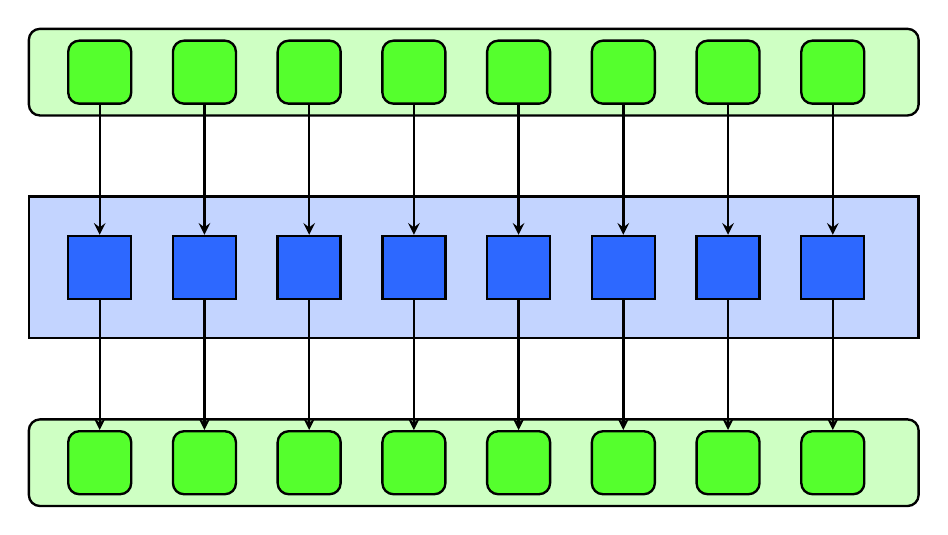
\begin{tikzpicture}[
inputnode/.style={rounded corners, draw=black!100, fill=inputgreen!100, line width=0.3mm, minimum size=8mm},
input_output_substain/.style={rounded corners, draw=black!100, fill=inputsubstaingreen!100, line width=0.3mm, minimum width=11.3cm, minimum height=11mm},
functionnode/.style={rectangle, draw=black!100, fill=functionblue!100, line width=0.3mm, minimum size=8mm},
function_substain/.style={rectangle, draw=black!100, fill=functionsubstainblue!100, line width=0.3mm, minimum width=11.3cm, minimum height=18mm},
arrow/.style={->, line width=0.3mm,>=stealth}
]
%Nodes
%Nodes inputs
\node[input_output_substain] 										(input_substain) {};

\node[inputnode, right=0.5cm of input_substain.west, anchor=west] 	(input_node_1) {};
\node[inputnode] 													(input_node_2) [right=0.5cm of input_node_1] {};
\node[inputnode] 													(input_node_3) [right=0.5cm of input_node_2] {};
\node[inputnode] 													(input_node_4) [right=0.5cm of input_node_3] {};
\node[inputnode] 													(input_node_5) [right=0.5cm of input_node_4] {};
\node[inputnode] 													(input_node_6) [right=0.5cm of input_node_5] {};
\node[inputnode] 													(input_node_7) [right=0.5cm of input_node_6] {};
\node[inputnode] 													(input_node_8) [right=0.5cm of input_node_7] {};

%Nodes function
\node[function_substain] 										(function_substain) [below=1cm of input_substain] {};

\node[functionnode, right=0.5cm of function_substain.west, anchor=west] 	(function_node_1) {};
\node[functionnode] 													(function_node_2) [right=0.5cm of function_node_1] {};
\node[functionnode] 													(function_node_3) [right=0.5cm of function_node_2] {};
\node[functionnode] 													(function_node_4) [right=0.5cm of function_node_3] {};
\node[functionnode] 													(function_node_5) [right=0.5cm of function_node_4] {};
\node[functionnode] 													(function_node_6) [right=0.5cm of function_node_5] {};
\node[functionnode] 													(function_node_7) [right=0.5cm of function_node_6] {};
\node[functionnode] 													(function_node_8) [right=0.5cm of function_node_7] {};

%Nodes outputs
\node[input_output_substain] 										(output_substain) [below=1cm of function_substain] {};

\node[inputnode, right=0.5cm of output_substain.west, anchor=west] 	(output_node_1) {};
\node[inputnode] 													(output_node_2) [right=0.5cm of output_node_1] {};
\node[inputnode] 													(output_node_3) [right=0.5cm of output_node_2] {};
\node[inputnode] 													(output_node_4) [right=0.5cm of output_node_3] {};
\node[inputnode] 													(output_node_5) [right=0.5cm of output_node_4] {};
\node[inputnode] 													(output_node_6) [right=0.5cm of output_node_5] {};
\node[inputnode] 													(output_node_7) [right=0.5cm of output_node_6] {};
\node[inputnode] 													(output_node_8) [right=0.5cm of output_node_7] {};


%Arrow
%Arrow from input to function
\draw [arrow] (input_node_1) -- (function_node_1);
\draw [arrow] (input_node_2) -- (function_node_2);
\draw [arrow] (input_node_3) -- (function_node_3);
\draw [arrow] (input_node_4) -- (function_node_4);
\draw [arrow] (input_node_5) -- (function_node_5);
\draw [arrow] (input_node_6) -- (function_node_6);
\draw [arrow] (input_node_7) -- (function_node_7);
\draw [arrow] (input_node_8) -- (function_node_8);

%Arrow from function to output
\draw [arrow] (function_node_1) -- (output_node_1);
\draw [arrow] (function_node_2) -- (output_node_2);
\draw [arrow] (function_node_3) -- (output_node_3);
\draw [arrow] (function_node_4) -- (output_node_4);
\draw [arrow] (function_node_5) -- (output_node_5);
\draw [arrow] (function_node_6) -- (output_node_6);
\draw [arrow] (function_node_7) -- (output_node_7);
\draw [arrow] (function_node_8) -- (output_node_8);

\end{tikzpicture}


\end{document}

